% Chapter 3

\chapter{Results} % Main chapter title
\label{Chapter3} % For referencing the chapter elsewhere, use \ref{Chapter3} 
\addtocontents{toc}{\setcounter{tocdepth}{1}}
\section{Assessment of inducible GLUT1 expression}
Previous results from the work of our laboratory showed that the GLUT1\textsuperscript{P485L} mutation leads to specific interaction with clathrins and internalization of the protein. In order to further investigate the role and functional effects of the mutation, we generated two Flp-In T-Rex HEK293 cell lines containing inducible BirA-FLAG epitope-tagged full length wild-type or mutant GLUT1 (Figure~\ref{fig:vectors}). The cells constitutively express Tet repressor (TetR) which binds to the TetO\textsubscript{2} sequence in the promoter of transgenic GLUT1~\cite{Hillen}. Upon addition, tetracycline binds to the TetR, causing the release of TetR from TetO\textsubscript{2} and induction of transgene transcription~\cite{Hillen}. In this thesis doxycycline was used as a relatively stable tetracycline derivative to induce the expression of the BirA-FLAG tagged GLUT1 variants~\cite{Xu}.

To determine the optimal conditions for inducible expression, GLUT1 wild-type and mutant cells were grown in different concentrations of doxycycline for 24 hr and the expression of the GLUT1 protein was analyzed by Western blotting with anti-FLAG antibody. Compared with 0.1 \textmu g/mL doxycycline, induction with 1 \textmu g/mL doxycycline resulted in higher GLUT1 levels in wild-type cells, whereas in mutant cells the GLUT1 expression was not significantly altered (Figure~\ref{fig:wb} A and C). The results showed that the lower dose of doxycycline was sufficient for induction of the system. 

Additionally, GLUT1 protein expression was quantified after 24 hr and 48 hr doxycycline induction. Further increase in the induction time did not result in increased GLUT1 levels in wild-type cells, but actually decreased the expression in mutant cells compared to the 24 hr time point (Figure~\ref{fig:wb} B and D). Therefore the induction with 0.1 \textmu g/mL doxycycline for 24 hr was selected in the following experiments to reduce toxic side effects of the drug~\cite{Zeltser}.

\begin{figure}[h]
\centering
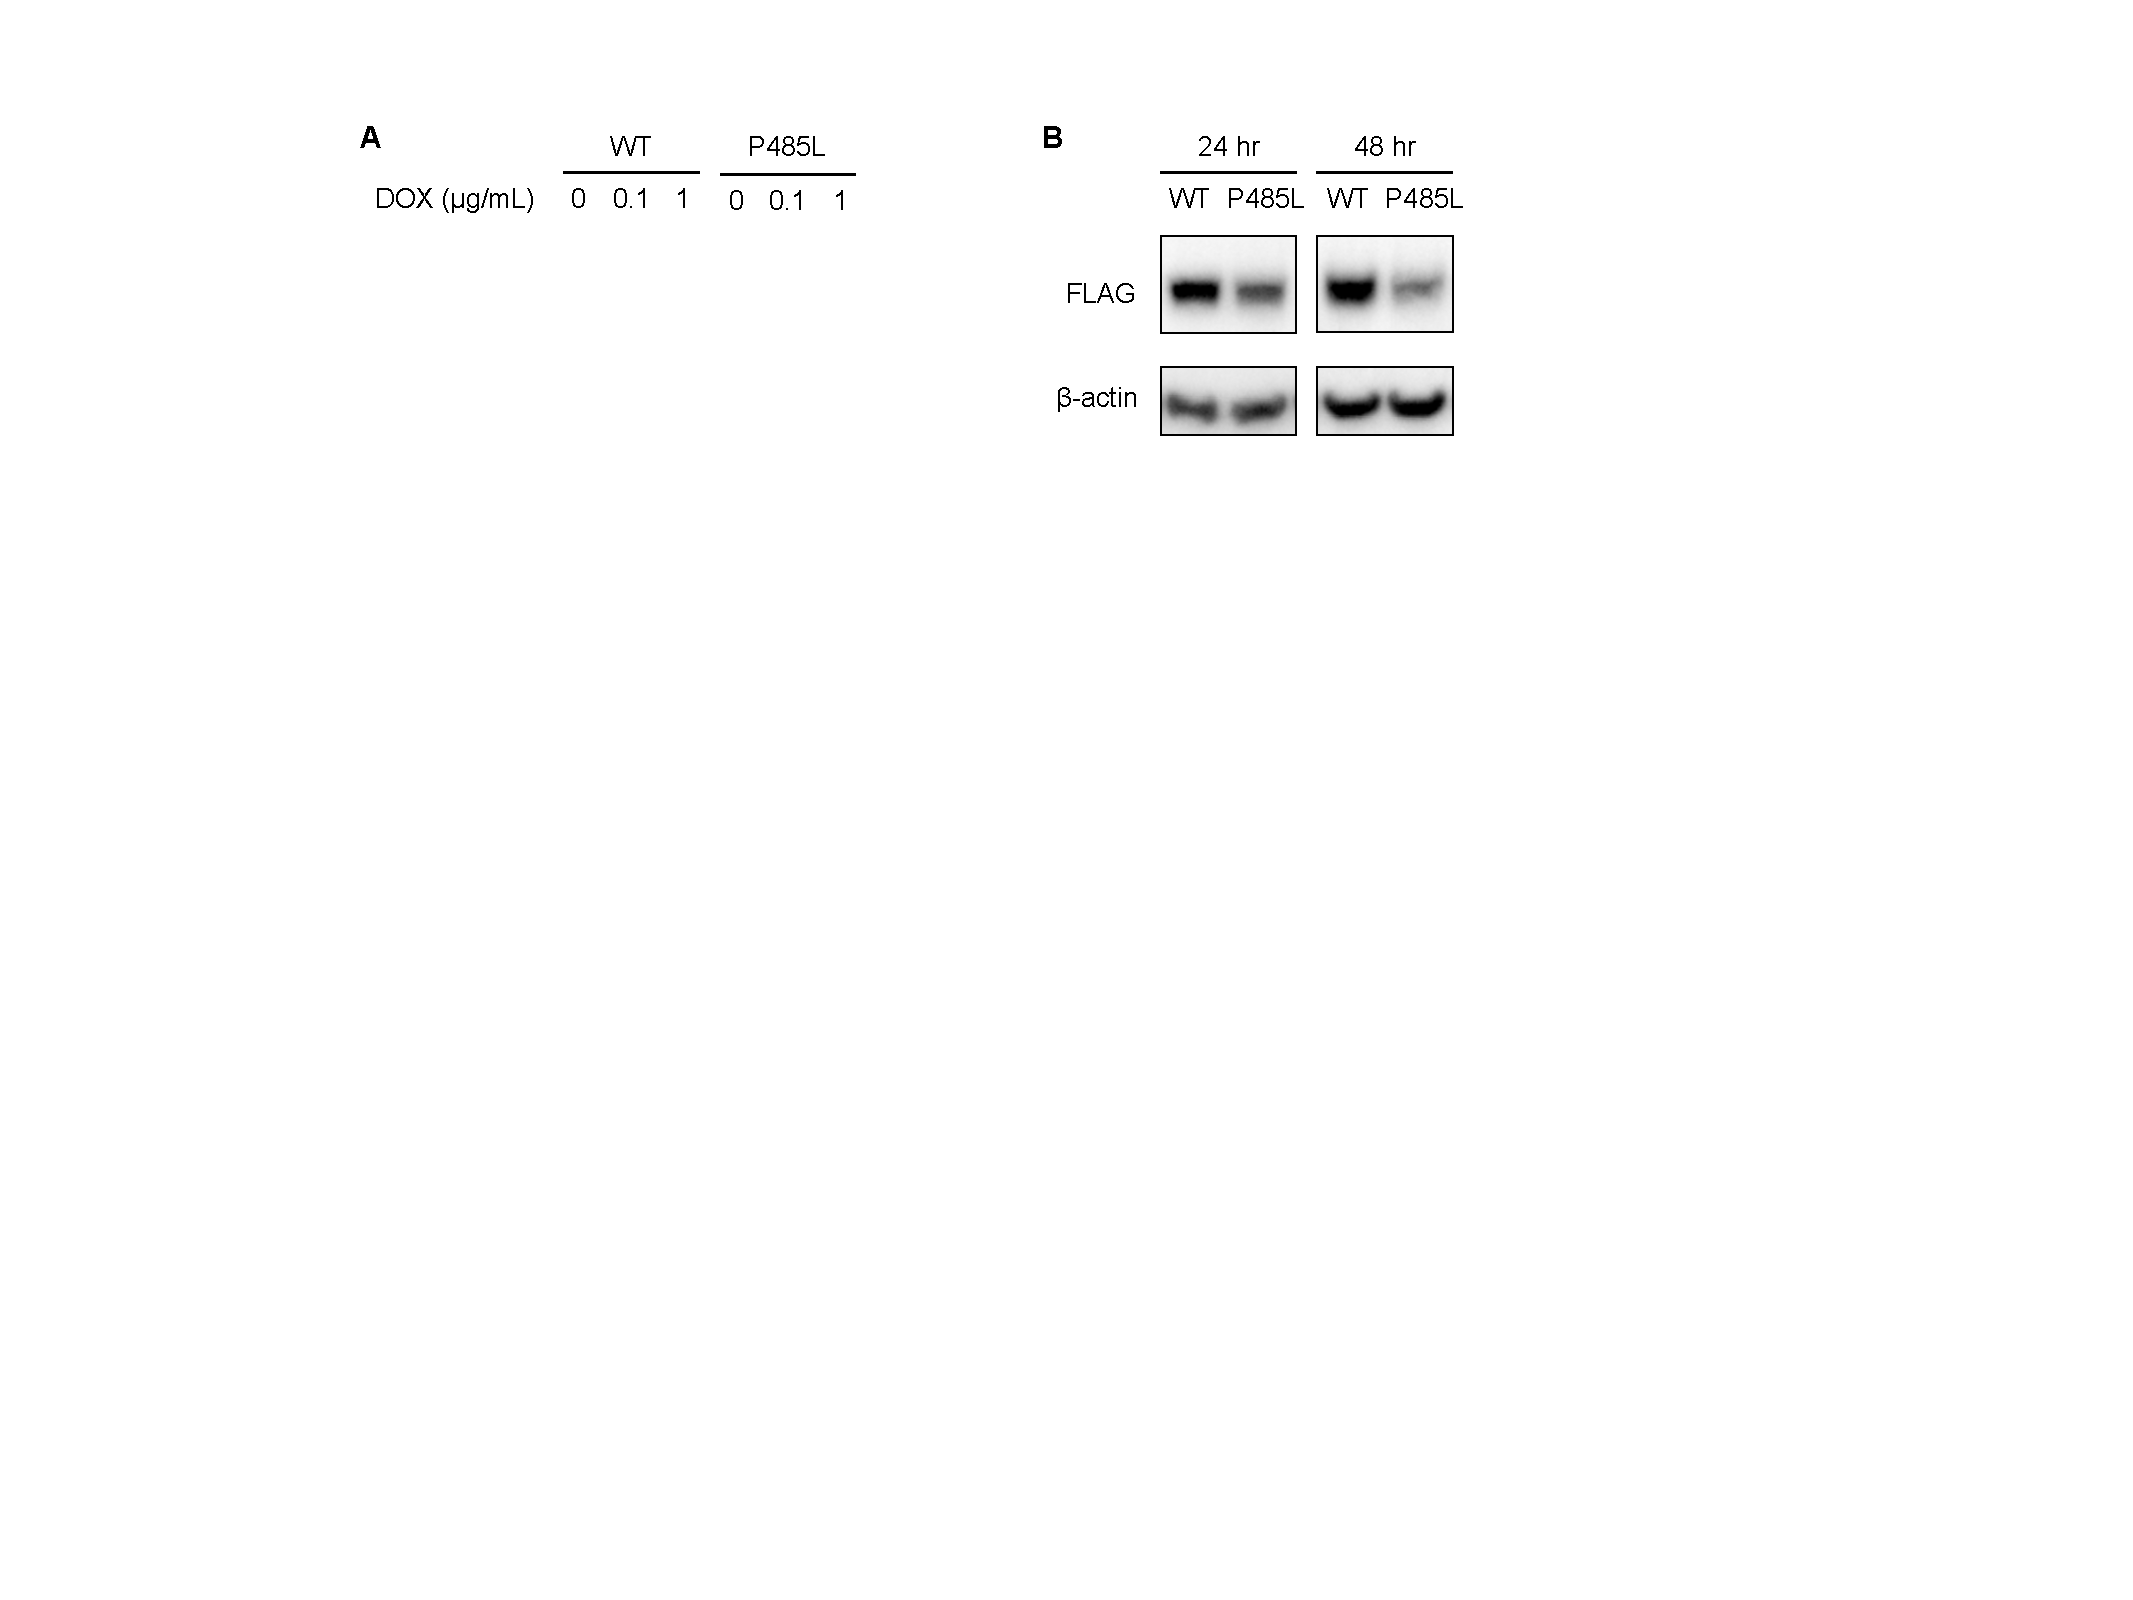
\includegraphics[scale=0.7]{Figures/WB}
\caption{The doxycycline-inducible expression of GLUT1 variants.}
%\smallskip
\vspace*{-3mm}
\small \justify
Different conditions were investigated to induce the expression of BirA-FLAG tagged GLUT1 with doxycycline. GLUT1 wild-type (WT) and mutant (P485L) cells were treated with varying concentrations of doxycycline (0, 0.1 or 1 \textmu g/mL) for 24 hr and analyzed with Western blotting (A, C). The inducible expression of GLUT1 was also compared between 24 hr and 48 hr induction with 0.1 \textmu g/mL doxycycline (B, D). Quantification of GLUT1 levels was achieved by normalizing to \textbeta -actin.
\label{fig:wb}
\end{figure}
% leakiness in expression, microscopy picture?
Furthermore, the doxycycline-inducible expression of GLUT1 was confirmed in confocal immunofluorescence microscopy experiments with a different anti-FLAG antibody. 
Although leakiness in expression was not detected in Western blotting, 

\begin{comment}
A low level of GLUT1 expression was observed in a small fraction of uninduced wild-type cells (Figure~\ref{fig:IF} A).
\begin{figure}[h]
\centering
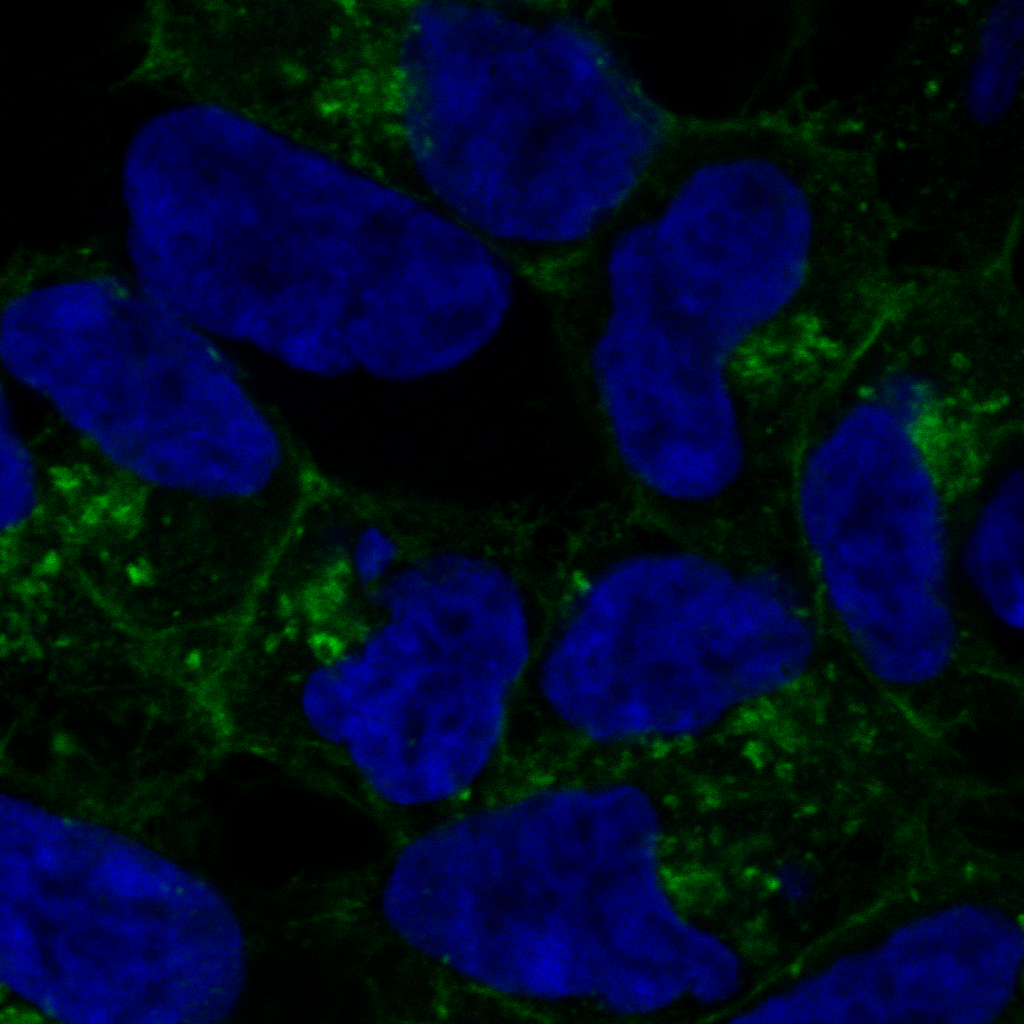
\includegraphics[scale=0.2]{Figures/induction_IF}
\caption{The inducible expression and localization of GLUT1 variants.}
\vspace*{-3mm}
\small \justify
The expression of GLUT1 was assessed by immunofluorescence microscopy. GLUT1 wild-type (WT) and mutant (P485L) cells were cultured on coverslips for 24 hr either in the absence or presence of 0.1 {}\textmu g/mL doxycycline. Immunostaining was performed with monoclonal mouse anti-FLAG and Alexa 488-conjugated anti-mouse antibodies. A small subpopulation of uninduced wild-type cells showed weak expression of GLUT1 (A)
\label{fig:IF}
\end{figure}
%As expected, ARF localized to nucleolar regions (the compact circular regions of higher intensity as pointed by the arrow in panel A) while HA-RBP1 demonstrated strong nuclear localization with nucleolar exclusion, as shown by the dark nucleolar regions in panel B. Panel C confirms that RBP2 is localized exclusively to the nucleus. Panel D illustrates that the rabbit polyclonal ?-RBP2 antibody cannot be used in immunofluorescence because of the high amount of non-specific background signal it produces. Trials were done at various dilutions but all were negative and produced the same non-specific noise (data not shown). 
\end{comment}

\section{Inhibition of protein degradation}
%we examined LC3-II or p62 levels in serum-starved cellseither in the absence, or presence of bafilomycin A1, an agent thatinhibits lysosomal acidification and/or inhibits autophagosome-lysosome fusion; this treatment leads to reduced degradation andhence, accumulation of autophagy substrates A Role for Presenilins in Autophagy Revisited: Normal Acidification of Lysosomes in Cells Lacking PSEN1 and PSEN2 (PDF Download Available). Available from: https://www.researchgate.net/publication/227858130_A_Role_for_Presenilins_in_Autophagy_Revisited_Normal_Acidification_of_Lysosomes_in_Cells_Lacking_PSEN1_and_PSEN2 [accessed Jul 13, 2017].
%LC3-II levels were elevated in cultured WT-ES cells(Fig. 1A, compare lanes 1, 2)

%~\cite{Yamamoto,Tanida,Klionsky}

\section{Proximity labeling of GLUT1 variants}

\section{Co-localization study of GLUT1 variants}
\begin{figure}[h]
\centering
\includegraphics[scale=0.7]{Figures/tf}
\caption{The mutant GLUT1 co-localizes with endocytosed transferrin.}
\vspace*{-3mm}
\small \justify
But not the wild-type GLUT1.
\label{fig:tf}
\end{figure}

\begin{figure}[h]
\centering
\includegraphics[scale=0.7]{Figures/tf2}
\caption{The mutant GLUT1 co-localizes with endocytosed transferrin.}
\vspace*{-3mm}
\small \justify
The colorful version
\label{fig:tf2}
\end{figure}
%----------------------------------------------------------------------------------------
% Define some commands to keep the formatting separated from the content 
